\documentclass{standalone}

%----------------------------------------------------------------------------------------------%
%                                 Packages and basic declarations
%----------------------------------------------------------------------------------------------%

\usepackage[utf8]{inputenc}
\usepackage{pgfplots}
\usepackage{tikz}


%----------------------------------------------------------------------------------------------%
%----------------------------------------------------------------------------------------------%
%                                            DOCUMENT STARTS
%----------------------------------------------------------------------------------------------%
%----------------------------------------------------------------------------------------------%

\begin{document}


%Tikz picture starts%

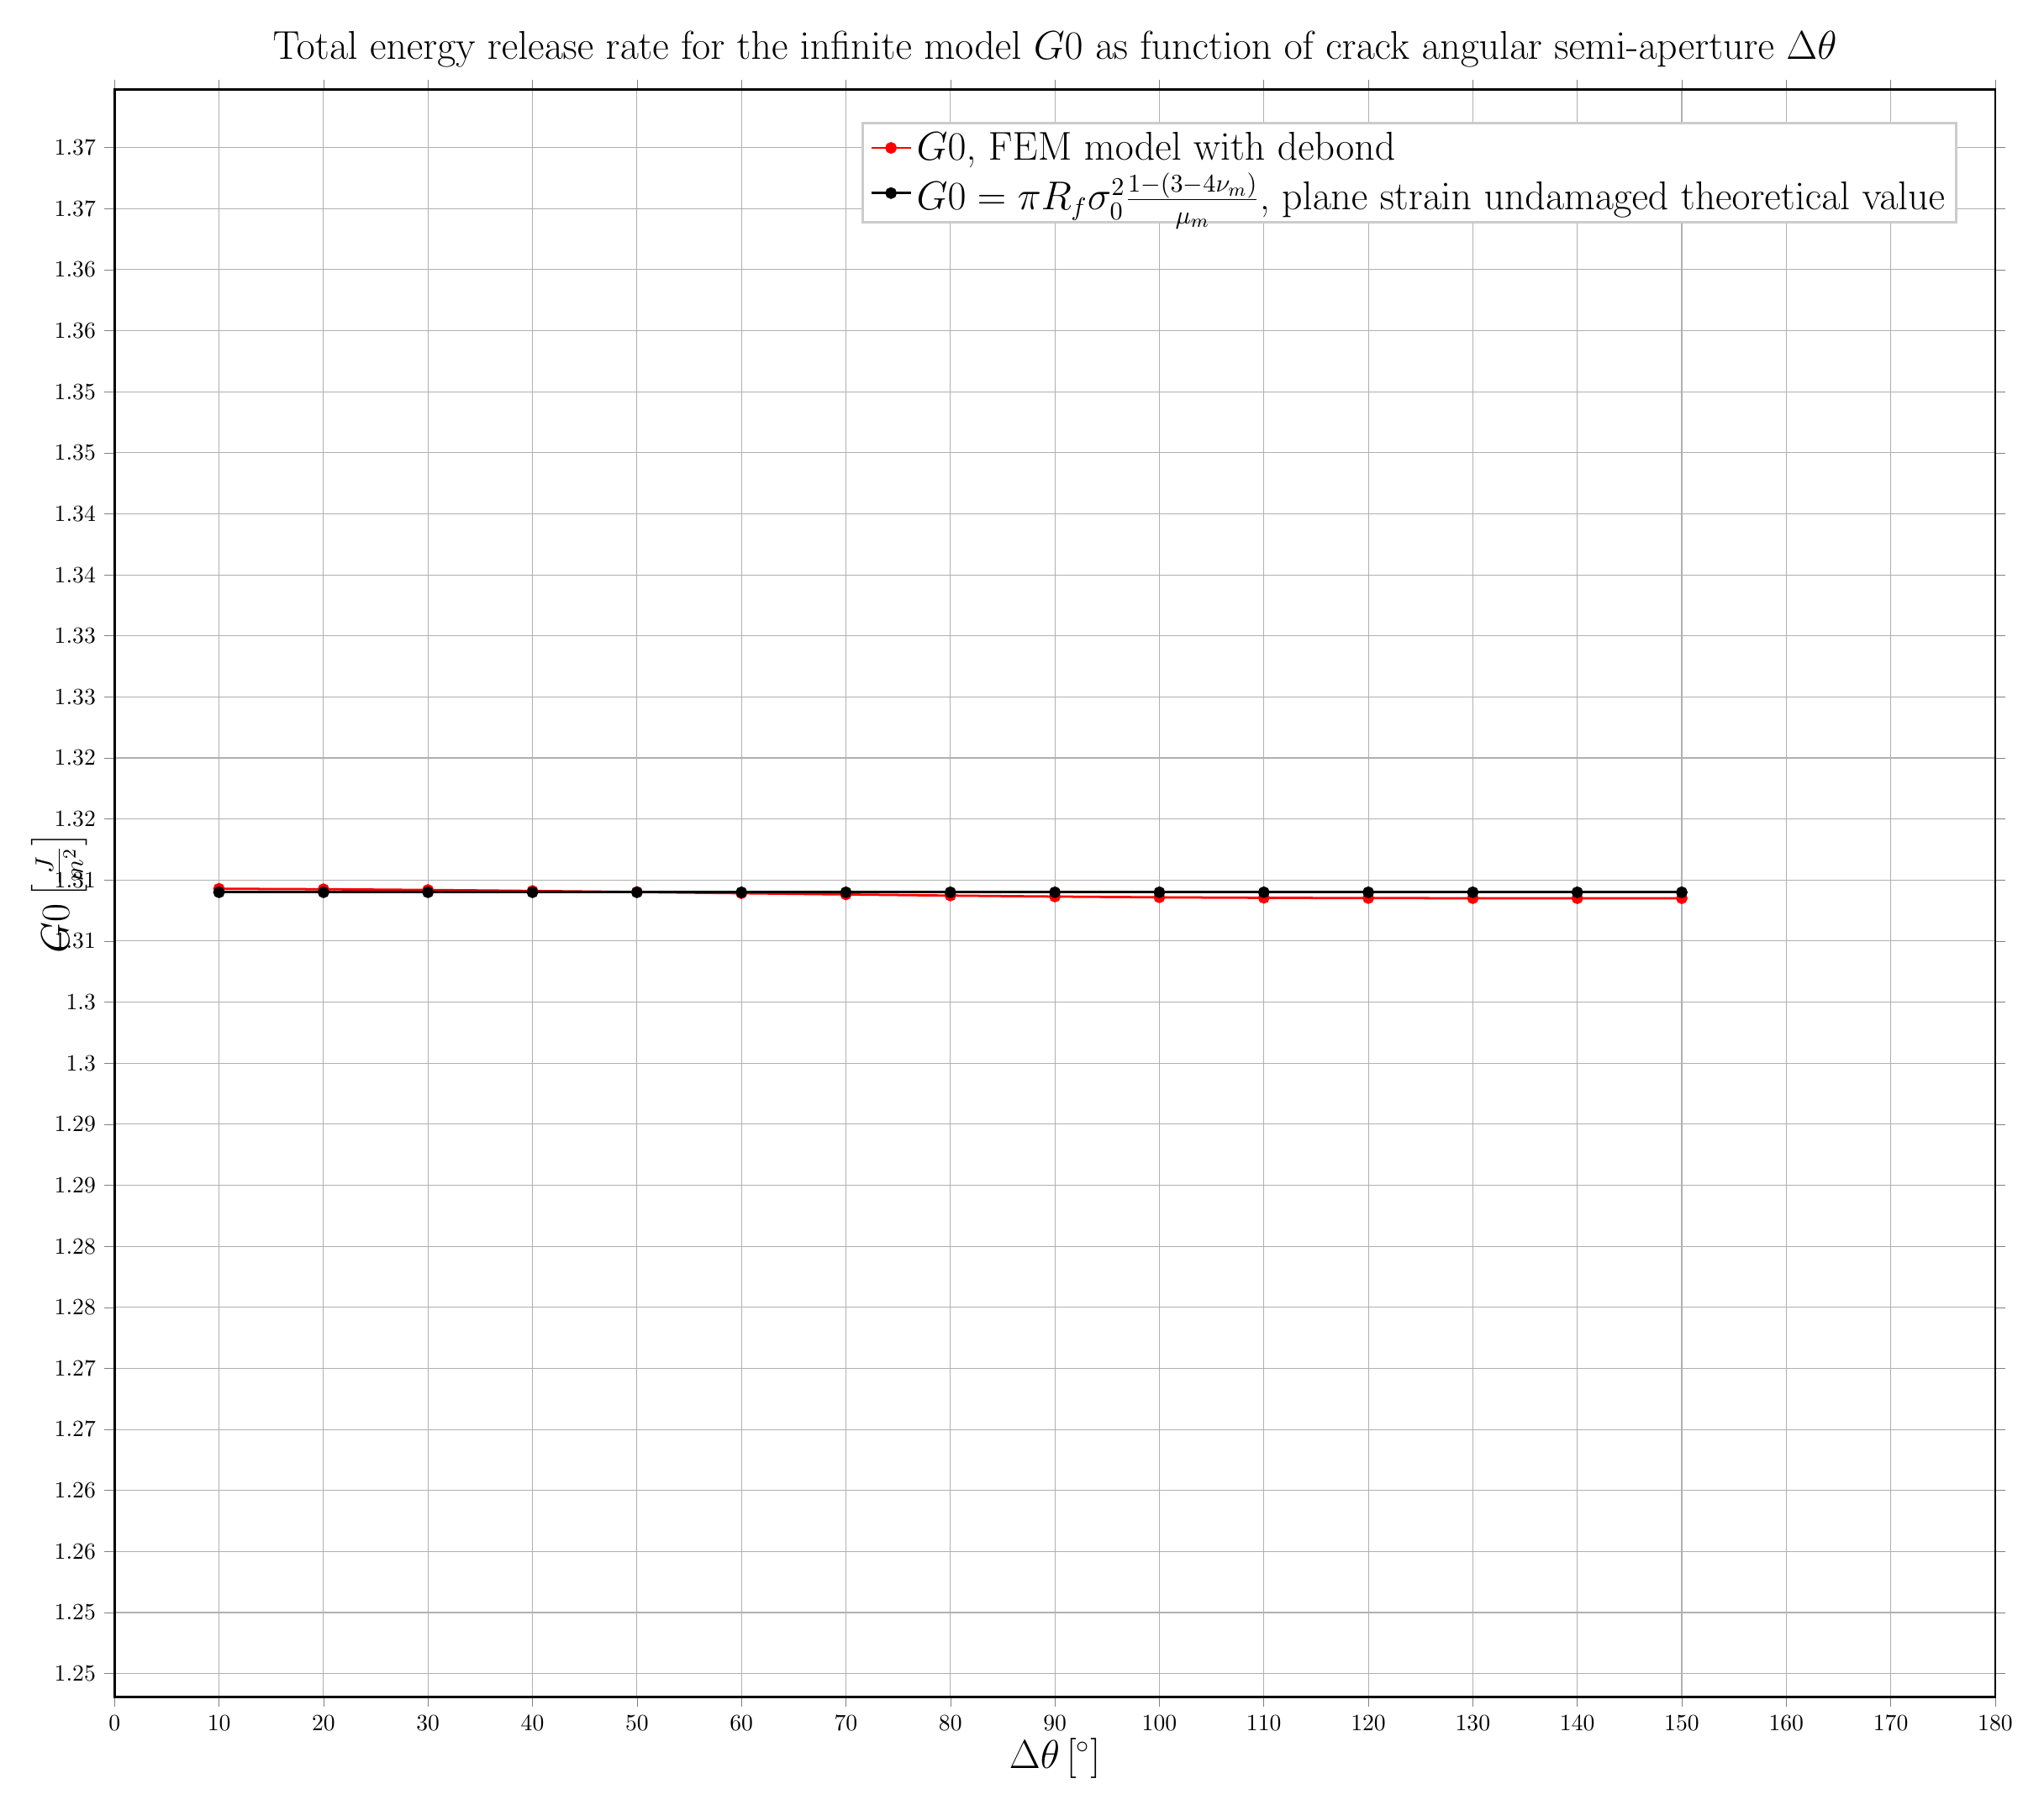
\begin{tikzpicture}

%Tikz axis starts%

\begin{axis}[width=30cm,
title={Total energy release rate for the infinite model $G0$ as function of crack angular semi-aperture  $\Delta\theta$},
title style={font=\fontsize{16}{8}\selectfont},
xlabel style={at={(axis description cs:0.5,-0.02)},anchor=north,font=\fontsize{16}{8}\selectfont},
ylabel style={at={(axis description cs:-0.01,.5)},anchor=south,font=\fontsize{16}{8}\selectfont},
xlabel={$\Delta\theta\left[^{\circ}\right]$},ylabel={$G0\left[\frac{J}{m^{2}}\right]$},
xmin=0.0,
xmax=180.0,
ymin=1.24308269896,
ymax=1.37474995122,
tick align=outside,
tick label style={font=\normalsize},
xtick={0.0,10.0,20.0,30.0,40.0,50.0,60.0,70.0,80.0,90.0,100.0,110.0,120.0,130.0,140.0,150.0,160.0,170.0,180.0},
xmajorgrids,
x grid style={lightgray!92.026143790849673!black},
ymajorgrids,
y grid style={lightgray!92.026143790849673!black},
line width=0.35mm,
legend style={draw=white!80.0!black,font=\fontsize{16}{12}\selectfont},
legend entries={{$G0$, FEM model with debond},{$G0=\pi R_{f}\sigma_{0}^{2}\frac{1-\left(3-4\nu_{m}\right)}{\mu_{m}}$, plane strain undamaged theoretical value}},
legend cell align={left}
]

\addplot[red,smooth,mark=*]
table{
10.0000799638 1.30928566783
20.0000438144 1.30924729336
29.9998676461 1.30918651176
40.0002686288 1.30910774245
49.9997304605 1.30901654023
60.0001314432 1.30891884996
69.9999586901 1.30882052882
79.9999225407 1.30872765155
90.0000025045 1.30864738267
100.000082468 1.30858562958
110.000046319 1.3085444149
119.999866736 1.30852152111
130.000274548 1.30851174288
139.999726135 1.30850911109
150.000133948 1.30850887968
};

\addplot[black,smooth,mark=*]
table{
10.0000799638 1.308996939
20.0000438144 1.308996939
29.9998676461 1.308996939
40.0002686288 1.308996939
49.9997304605 1.308996939
60.0001314432 1.308996939
69.9999586901 1.308996939
79.9999225407 1.308996939
90.0000025045 1.308996939
100.000082468 1.308996939
110.000046319 1.308996939
119.999866736 1.308996939
130.000274548 1.308996939
139.999726135 1.308996939
150.000133948 1.308996939
};

\end{axis}
%Tikz axis ends%


\end{tikzpicture}
%Tikz picture ends%


\end{document}

%----------------------------------------------------------------------------------------------%
%----------------------------------------------------------------------------------------------%
%                                            DOCUMENT ENDS
%----------------------------------------------------------------------------------------------%
%----------------------------------------------------------------------------------------------%

